\documentclass[12pt,oneside]{book}
\input{commoncommands}

%rename chapter headings
\renewcommand{\chaptername}{}
\renewcommand{\bibname}{References}

\usepackage{fancyhdr}
\pagestyle{fancy}
\lhead{}
\rhead{}
\chead{}
\renewcommand{\headrulewidth}{0pt}

\usepackage{draftwatermark}
\SetWatermarkText{DRAFT}
\SetWatermarkScale{1}

\begin{document}
\pagenumbering{gobble}
\bibliographystyle{unsrt}
	
\begin{minipage}[t][9in][s]{6.25in}

\headerB{
Impact of Fire Attack Utilizing \\
Interior and Exterior Streams on \\
Firefighter Safety and Occupant Survival: Howard Room Experiments \\
}

\normalsize

\headerC{
	{ \flushleft{
	Keith Stakes \\
	Robin Zevotek \\
	\vspace{0.2in}
	UL Firefighter Safety Research Institute \\
	Columbia, MD 20145 \\
	\vspace*{2\baselineskip}

	} 

	\vfill

	\flushright{

	\includegraphics[width=2.0in]{Figures/General/FSRI_GraphicShield.pdf} \\ [.3in]

	}
	}
	}

\end{minipage}

\newpage
\hspace{5in}
\newpage

\frontmatter

\begin{minipage}[t][9in][s]{6.25in}
\pagenumbering{gobble}


\headerB{
Impact of Fire Attack Utilizing \\
Interior and Exterior Streams on\\ 
Firefighter Safety and Occupant \\
Survival: Air Entrainment\\
}

\headerC{
\flushleft{
Keith Stakes \\
Robin Zevotek \\
\vspace{0.2in}
{UL Firefighter Safety Research Institute \\
Columbia, MD 21045 \\}}

\flushleft{\today \\}
}


\vfill

\flushright{\includegraphics[width=2in]{Figures/General/FSRI_GraphicShield.pdf}}

\titlesigs

\end{minipage}

\frontmatter

\section{Instrumentation}
Throughout this project measurements were taken of temperature, heat flux, pressure, gas velocity, and heat release rate. The same instrumentation was utilized for all three sets of experiments. The following describes the instrumentation used and potential uncertainty.

Heat flux measurements were made using 2.54 cm nominal diameter water-cooled Schmidt- Boelter heat flux gauges (Figure \ref{fig:HeatFluxGauge}). The gauges measured the combined radiative and convective heat flux. For these experiments, the dominant form of heat flux is radiative due to the distance of the heat flux gauges from the flames. It should be noted that the convective contribution to the heat flux is dependent upon the surface temperature of the heat flux gauge. The manufacturer gives an uncertainty of ±3\% and results from a study on heat flux calibration found the typical expanded uncertainty to be ±8\% \cite{HeatFluxRoundRobin}.

\begin{figure} [H]
	\centering
	\includegraphics[width = 3.5in]{0_Images/Instrumentation/Heat_Flux_Gauge.jpg}
	\caption{Water Cooled Schmidt-Boelter Heat Flux Gauge}
	\label{fig:HeatFluxGauge}
\end{figure}

Temperatures were recorded using a bare-bead, Chromel-Alumel (type K) thermocouple with a 0.5 mm nominal diameter (Figure \ref{fig:Thermocouple}). The uncertainty given by the manufacturer for the temperature measurements is ±2.2 $^{\circ}$C for temperatures below 293 $^{\circ}$C and ±0.75\% for higher temperatures \cite{TemperatureHandbook}. The thermocouple readings will be lower than the air temperature when the thermocouple is in the flame region, due to radiative losses to the surrounding cooler environment. When the thermocouples are farther from the flame region, the impact of radiation will result in temperature readings higher than the air temperature. Due to the effect of radiative heat transfer to the thermocouples, the expanded uncertainty is approximately ±15\%.

\begin{figure} [H]
	\centering
	\includegraphics[width = 4in]{0_Images/Instrumentation/Thermocouple.jpg}
	\caption{Chromel-Alumel (Type K) Thermocouple}
	\label{fig:Thermocouple}
\end{figure}

Pressure was recorded through the use of a Setra Model 264 differential pressure transducer with a range of $\pm$0.5in WC ($\pm$124.5 Pa) (Figure \ref{fig:Setra}). The transducer was used to evaluate the pressure difference from ambient pressure. The uncertainty given by the manufacturer is $\pm$\%0.005 in WC or $\pm$1.2 Pa \cite{SetraManual}.

\begin{figure} [H]
	\centering
	\includegraphics[width = 3in]{0_Images/Instrumentation/Setra.jpg}
	\caption{Setra Model 264 Differential Pressure Transducer}
	\label{fig:Setra}
\end{figure}

Gas velocities were obtained through the use of a bi-directional probe in conjunction with a differential pressure transducer and iconel thermocouple. The probe was constructed of stainless steel. The iconel thermocouple was a 0.063in. (1.6 mm) diameter type KSL iconel 600 sheathed grounded junction with a type K, 24 gauge glass/glass insulation lead. The differential pressure transducer was a Setra Model 264 with a range of $\pm$1.0in. WC ($\pm$248.8 Pa). The configuration had a velocity range of $\pm$54 mph ($\pm$24.2 m/s). The pressure transducers were configured in groups of 6, contained in a single plastic box with connections for pressure, temperature and power (Figure \ref{fig:BDP}b). Five probes were installed in openings where velocity measurements were taken, centered horizontally in the opening (Figure \ref{fig:BDP}a). Velocity measurement with this configuration was determined to have an uncertainty of $\pm$5\% \cite{BDPInPoolFires}.

\begin{figure} [H]
	\centering
	\begin{tabular}{c c}
		\subfloat[Pressure Transducer Box]{\includegraphics[height = 2.5in]{0_Images/Instrumentation/PressureBox.jpg}} &
		\subfloat[Bi-Directional Probe Array]{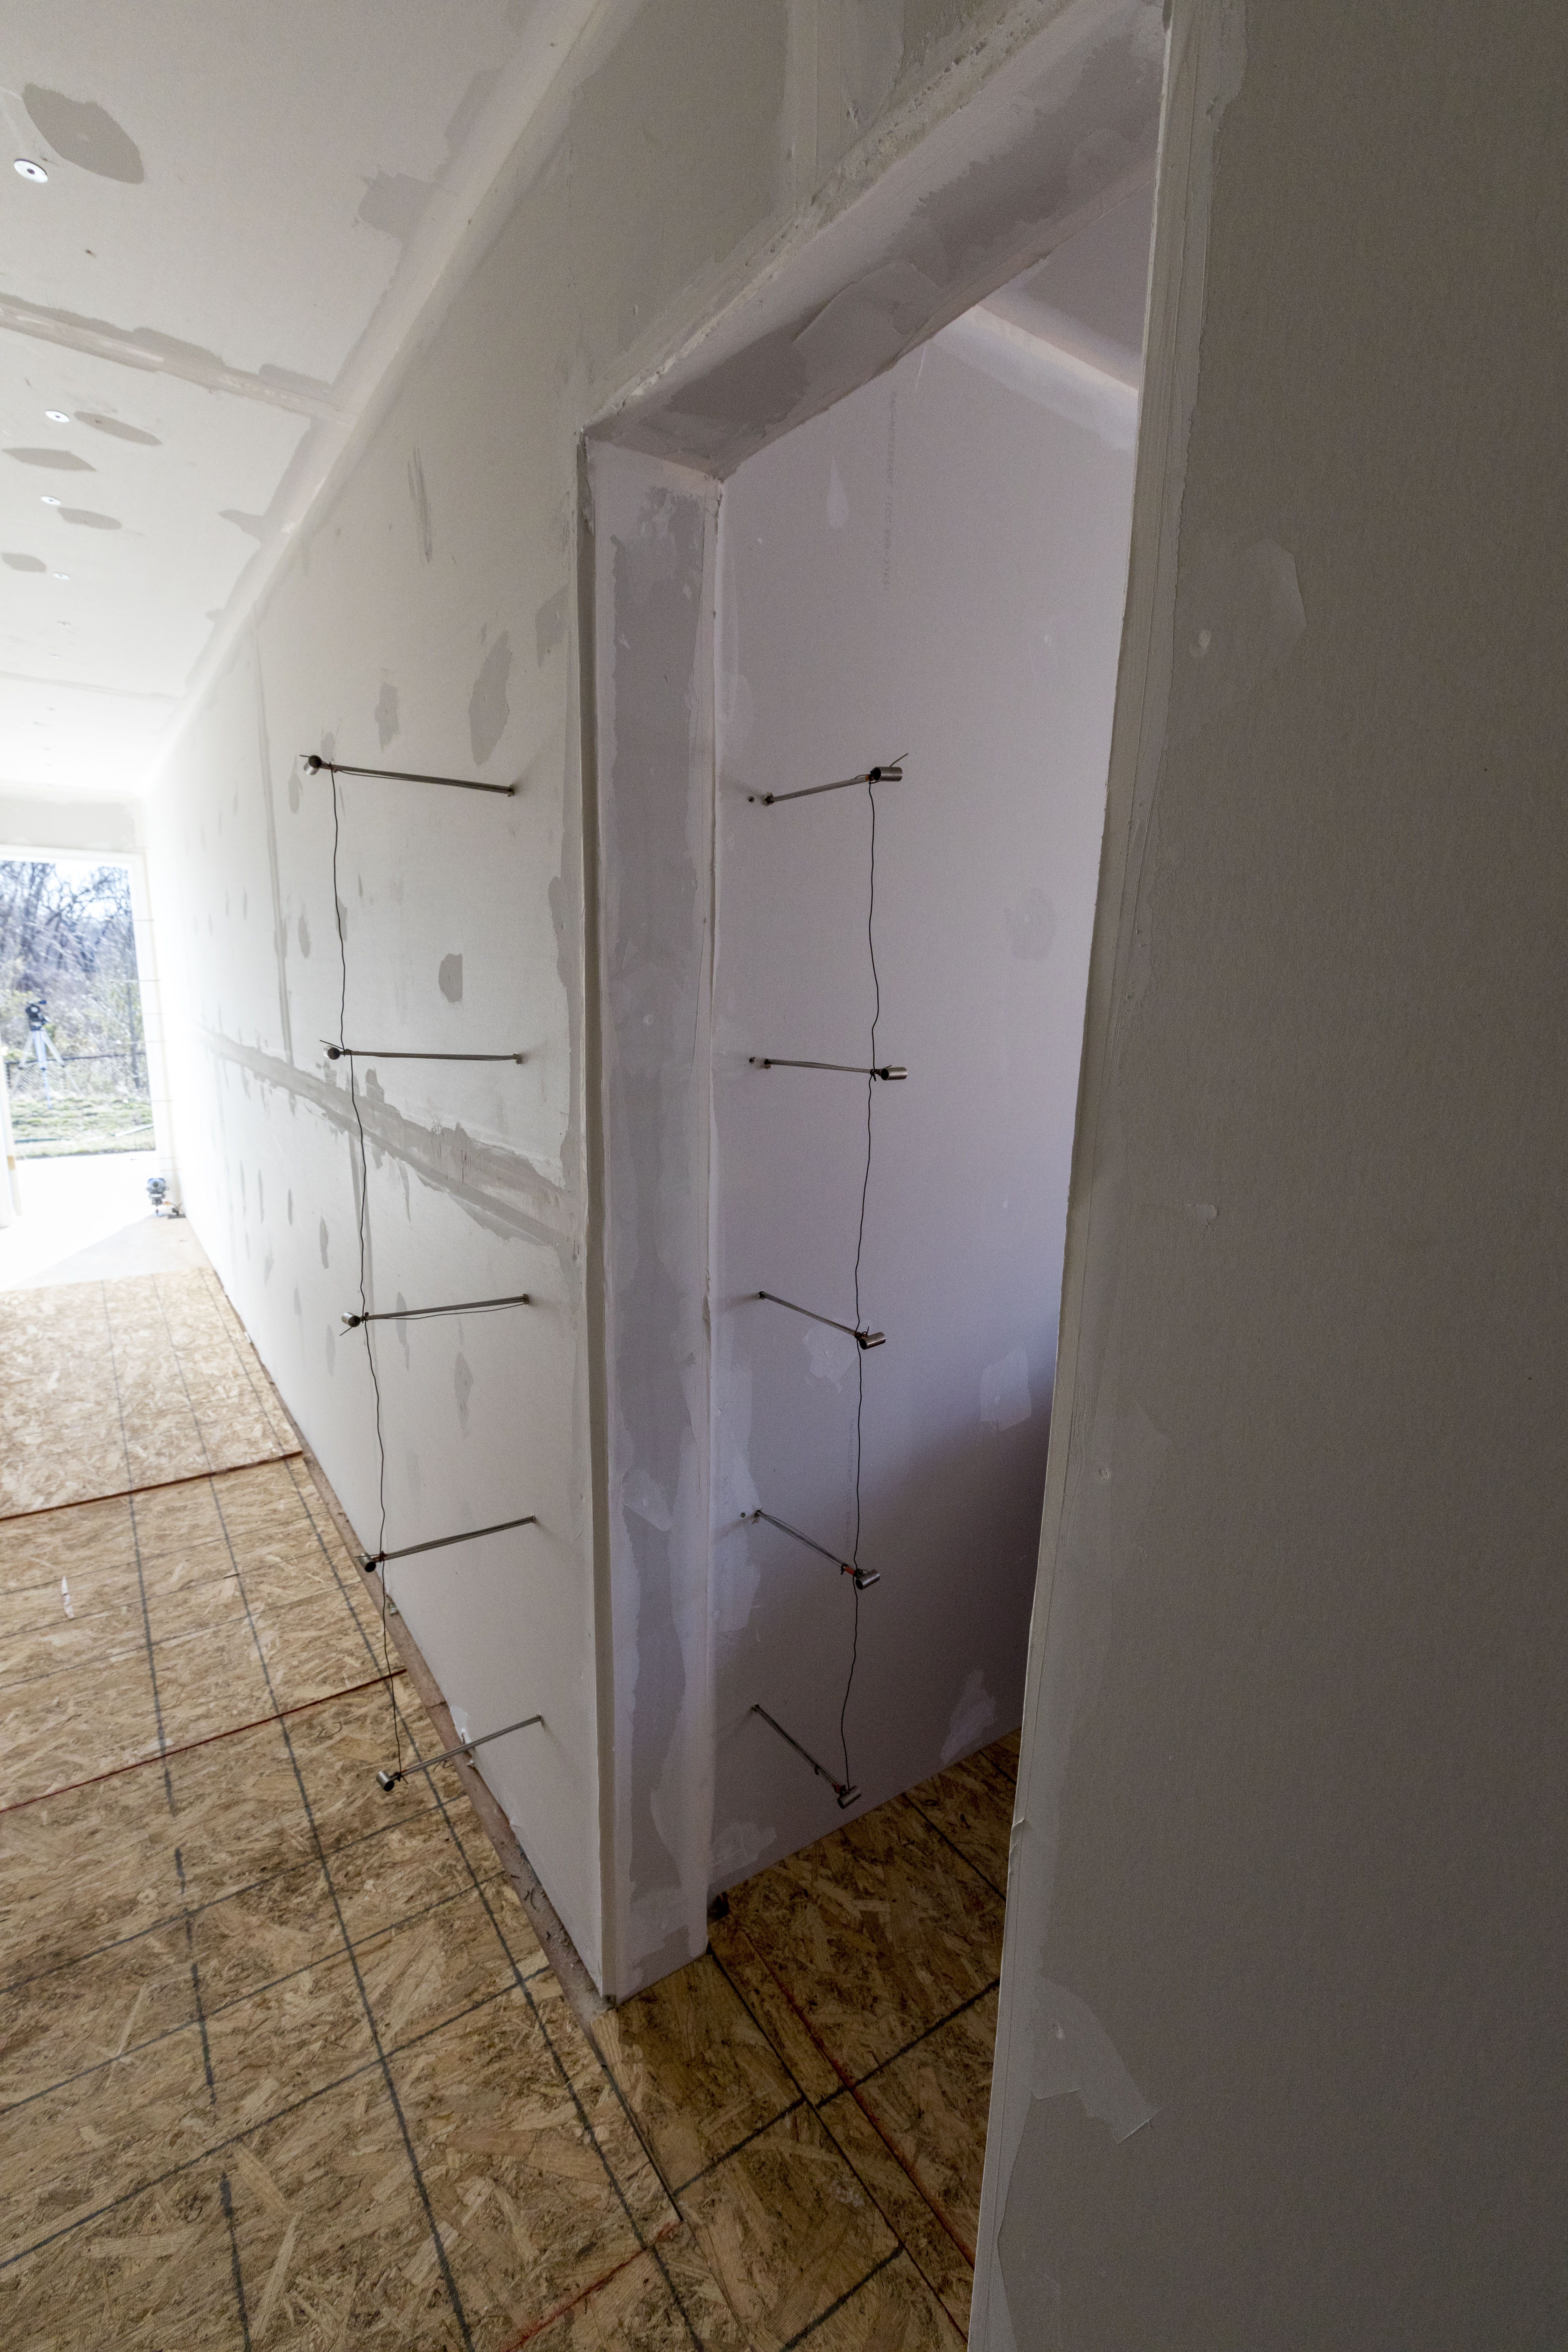
\includegraphics[height = 2.5in]{0_Images/Instrumentation/BDPArray.jpg}} \\
	\end{tabular}
	\caption{Bi-Directional Probe}
	\label{fig:BDP}
\end{figure}

The heat release rate is measured through the use of oxygen consumption techniques. The oxygen consumption calorimeter is capable of accurately measuring the heat release rate up to 10 MW. Above 10 MW, larger inaccuracies are expected due to the combustion products overflowing the collection hood. Figure \ref{fig:Hood} shows the collection hood utilized for the calorimetry data.

\begin{figure} [H]
	\centering
	\includegraphics[width = 5in]{0_Images/Instrumentation/Calorimetry_hood.jpg}
	\caption{Oxygen Consumption Calorimetry Hood}
	\label{fig:Hood}
\end{figure}

Standard video was obtained through the use of Bosch VTC-206F03-4 video cameras (Figure \ref{fig:BullettCam}). Thermal imaging of the front and rear of the structure was taken using ISG Infrasys Elite XR (Figure \ref{fig:IRCam}). The thermal imaging camera has a fixed emissivity value of 0.9 and was utilized for visual representation of relative conditions, no temperature measurements or analysis were derived using the camera. All cameras were recorded using a TriCaster 8200 video acquisition system.

\begin{figure} [H]
	\centering
	\includegraphics[width = 3in]{0_Images/Instrumentation/BullettCam.jpg}
	\caption{Bosch VTC-206F03-4 Video Camera}
	\label{fig:BullettCam}
\end{figure}

\begin{figure} [H]
	\centering
	\includegraphics[width = 2.5in]{0_Images/Instrumentation/ISG_IR.jpg}
	\includegraphics[width = 2.5in]{0_Images/Instrumentation/ISG_IR2.jpg}
	\caption{ISG Elite XR Fire Service Thermal Imaging Camera}
	\label{fig:IRCam}
\end{figure}

Gas samples were analyzed through the use of OxyMat6 and UltraMat23 Siemens gas analyzers. Samples were pulled from the structure through the use of cole palmer model L-79200-30 vacuum/pressure diaphragm pump rated at 0.75CFM via a stainless steel tube. The sample is filtered through a coarse filter, solberg model 842, 2 micron paper filter before running through a condensing trap to remove moisture. The sample then runs through a drying tube dry fine filter, perma pure model FF-250-SG-2.5G with a 1 micron filter FF-250-E-2.5G before splitting into two branches and entering the UltraMat and OxyMat analyzer. The analyzers are calibrated to measure CO from 0-50000PPM, CO2 from 0-20\% and O$_2$ from 0-25\%. 

\begin{figure}[H]
	\centering
	\begin{tabular}{*3c}
		\subfloat[Sample Line]{\includegraphics[width = 2in]{0_Images/Instrumentation/Gas_Analyzer/SamplePoint.jpg}} &
		\subfloat[Vaccum Pump - Cole Palmber L-79200-30]{\includegraphics[width = 2in]{0_Images/Instrumentation/Gas_Analyzer/VaccumPump.jpg}} &
		\subfloat[Coarse Filter - Solberg 842]{\includegraphics[width = 2in]{0_Images/Instrumentation/Gas_Analyzer/CourseFilter.jpg}} \\
		\subfloat[Condensing Tube]{\includegraphics[height = 2in]{0_Images/Instrumentation/Gas_Analyzer/CoilCondenser.png}} &
		\subfloat[Dririte Tube]{\includegraphics[height = 2in]{0_Images/Instrumentation/Gas_Analyzer/DriRightTube.jpg}} &
		\subfloat[Fine Filter - Perma Pure FF-250-SG-2.5G]{\includegraphics[height = 2in]{0_Images/Instrumentation/Gas_Analyzer/FineFilter.jpg}} \\
	\end{tabular}
	\subfloat[Gas Analyzers]{\includegraphics[width = 2in]{0_Images/Instrumentation/Gas_Analyzer/GasAnalyzers.jpg}}
	\caption{Gas Analyzer Configuration}
	\label{fig:GasAnalyzers}
\end{figure}

All data was logged through the use of a national instruments data acquisition system incorporating a SCXI-1001 chassis with 8 SCXI-1102C 32-Channel modules (Figure \ref{fig:DataSystem}). The system is configured for a total of 256 channels capable of reading values between 0-10 volts DC. Values are recorded once a second and translated to quantities of interest through the use of LabVIEW software specifically programmed for use with the system.

\begin{figure}[H]
	\centering
	\includegraphics[width = 4in]{0_Images/Instrumentation/DataSystem.jpg}
	\caption{Data Acquisition System}
	\label{fig:DataSystem}
\end{figure}

\clearpage

\section{Test Descriptions}

\paragraph{Experiment 1} \mbox{}

Experiment 1 was a room and contents fire in the bedroom of the structure testing the ability for the fire to regrow after an exterior attack. The door to the hallway and the bedroom window within the structure were open for the duration of the test. The fire was allowed to grow to steady state before suppression. Suppression was conducted from the exterior of the structure via a straight stream on a 150~gpm at 75~psi combination nozzle connected to a 1~3/4~in hoseline. The nozzle firefighter was positioned close to the window opening and the hose stream was directed at the ceiling via a max angle position. Water was applied for approximately 10 seconds. Figure \ref{fig:Exp1Config} shows the configuration of the structure and Table \ref{Table:Exp1Interventions} shows at what times interventions were performed. 

% The results of Experiment 1 can be found in Appendix \ref{App:Exp1Results}. To view the full experiment video \href{https://youtu.be/gl8rc1Nsl1k}{Click Here}.

\begin{figure}[H]
	\centering
	\includegraphics[width=5in]{Howard_Exp_1.png}
	\caption{Experiment 1 Configuration}
	\label{fig:Exp1Config}
\end{figure}

\begin{table}[H]
	\centering
	\caption{Experiment 1 Interventions}
	\begin{tabular}{|c|c|} 
		\hline
		Time & Intervention \\ \hline \hline
		00:00 & Ignition - Bedroom \\ \hline
		04:30 & Exterior Suppression \\ \hline
		13:00 & End Experiment\\ \hline
	\end{tabular}
	\label{Table:Exp1Interventions}
\end{table}

\clearpage

\paragraph{Experiment 2} \mbox{}

Experiment 2 was a room and contents fire in the bedroom of the structure testing the ability for the fire to regrow after an exterior attack. This test was similar to Experiment 1 with the exception of additional fuel loading in the fire room. The details of the differences in the fuel loading can be found in the Fuel Load section above. The door to the hallway and the bedroom window within the structure were open for the duration of the test. The fire was allowed to grow to steady state before suppression. Suppression was conducted from the exterior of the structure via a straight stream on a 150~gpm at 75~psi combination nozzle connected to a 1~3/4~in hoseline. The nozzle firefighter was positioned close to the window opening and the hose stream was directed at the ceiling via a max angle position. Water was applied for approximately 10 seconds. After 16 minutes, it was determined that the fire was not going to re-grow and thus was re-ignited manually in the bedroom and was allowed to grow uninhibited once again until a steady state condition was reached. Exterior suppression was completed as before with water flowing for approximately 8 seconds. After approximately 14 minutes, the fire re-grew to a new steady state and was suppressed one last time using the same method as above with water flowing for approximately 10 seconds. Figure \ref{fig:Exp2Config} shows the configuration of the structure and Table \ref{Table:Exp2Interventions} shows at what times interventions were performed.  

% The results of Experiment 1 can be found in Appendix \ref{App:Exp1Results}. To view the full experiment video \href{https://youtu.be/gl8rc1Nsl1k}{Click Here}.

\begin{figure}[H]
	\centering
	\includegraphics[width=5in]{Howard_Exp_2.png}
	\caption{Experiment 2 Configuration}
	\label{fig:Exp2Config}
\end{figure}

\begin{table}[H]
	\centering
	\caption{Experiment 2 Interventions}
	\begin{tabular}{|c|c|} 
		\hline
		Time & Intervention \\ \hline \hline
		00:00 & Ignition - Bedroom \\ \hline
		05:00 & Exterior Suppression \\ \hline
		21:00 & Second Ignition - Bedroom \\ \hline
		27:00 & Exterior Suppression \\ \hline
		40:20 & Exterior Suppression \\ \hline
		44:00 & End Experiment\\ \hline
	\end{tabular}
	\label{Table:Exp2Interventions}
\end{table}

\clearpage

\paragraph{Experiment 3} \mbox{}

Experiment 3 was a room and contents fire in the bedroom of the structure testing the impact of hose stream air entrainment on fire behavior and suppression capability. The door to the hallway and the bedroom window within the structure were open for the duration of the test. The fire was allowed to grow to steady state before suppression. Suppression was conducted from the interior of the structure via a straight stream on a 150~gpm at 75~psi combination nozzle connected to a 1~3/4~in hoseline. The nozzle firefighter advanced down the hallway and the hose stream was directed ahead in a wall-ceiling-wall pattern before entering the fire room for final extinguishment. Figure \ref{fig:Exp3Config} shows the configuration of the structure and Table \ref{Table:Exp3Interventions} shows at what times interventions were performed.  

% The results of Experiment 1 can be found in Appendix \ref{App:Exp1Results}. To view the full experiment video \href{https://youtu.be/gl8rc1Nsl1k}{Click Here}.

\begin{figure}[H]
	\centering
	\includegraphics[width=5in]{Howard_Exp_3.png}
	\caption{Experiment 3 Configuration}
	\label{fig:Exp3Config}
\end{figure}

\begin{table}[H]
	\centering
	\caption{Experiment 3 Interventions}
	\begin{tabular}{|c|c|} 
		\hline
		Time & Intervention \\ \hline \hline
		00:00 & Ignition - Bedroom \\ \hline
		05:00 & Interior Suppression \\ \hline
		15:00 & End Experiment\\ \hline
	\end{tabular}
	\label{Table:Exp3Interventions}
\end{table}

\clearpage

\paragraph{Experiment 4} \mbox{}

Experiment 4 was a room and contents fire in the bedroom of the structure testing the impact of hose stream air entrainment on fire behavior and suppression capability. The door to the hallway and the bedroom window within the structure were open for the duration of the test. The fire was allowed to grow to steady state before suppression. Suppression was conducted from the interior of the structure via a narrow fog stream on a 150~gpm at 75~psi combination nozzle connected to a 1~3/4~in hoseline. The nozzle firefighter advanced down the hallway and the hose stream was directed ahead in an `O' pattern before entering the fire room for final extinguishment. Figure \ref{fig:Exp4Config} shows the configuration of the structure and Table \ref{Table:Exp4Interventions} shows at what times interventions were performed. 

% The results of Experiment 1 can be found in Appendix \ref{App:Exp1Results}. To view the full experiment video \href{https://youtu.be/gl8rc1Nsl1k}{Click Here}.

\begin{figure}[H]
	\centering
	\includegraphics[width=5in]{Howard_Exp_4.png}
	\caption{Experiment 4 Configuration}
	\label{fig:Exp4Config}
\end{figure}

\begin{table}[H]
	\centering
	\caption{Experiment 4 Interventions}
	\begin{tabular}{|c|c|} 
		\hline
		Time & Intervention \\ \hline \hline
		00:00 & Ignition - Bedroom \\ \hline
		07:30 & Interior Suppression \\ \hline
		14:00 & End Experiment\\ \hline
	\end{tabular}
	\label{Table:Exp4Interventions}
\end{table}

\clearpage

\paragraph{Experiment 5} \mbox{}

Experiment 5 was a room and contents fire in the bedroom of the structure testing the impact of door control. The bedroom window within the structure was open for the duration of the test. The fire was allowed to grow to steady state before the hall door was manipulated from the exterior of the structure. Several iterations of door open and door closed were performed before suppression. Suppression was conducted from the exterior of the structure via a straight stream on a 150~gpm at 75~psi combination nozzle connected to a 1~3/4~in hoseline. The nozzle firefighter was positioned close to the window opening and the hose stream was directed at the ceiling via a max angle position. Water was applied for approximately 10 seconds. Figure \ref{fig:Exp5Config} shows the configuration of the structure and Table \ref{Table:Exp5Interventions} shows at what times interventions were performed.

% The results of Experiment 1 can be found in Appendix \ref{App:Exp1Results}. To view the full experiment video \href{https://youtu.be/gl8rc1Nsl1k}{Click Here}.

\begin{figure}[H]
	\centering
	\includegraphics[width=5in]{Howard_Exp_5.png}
	\caption{Experiment 5 Configuration}
	\label{fig:Exp5Config}
\end{figure}

\begin{table}[H]
	\centering
	\caption{Experiment 5 Interventions}
	\begin{tabular}{|c|c|} 
		\hline
		Time & Intervention \\ \hline \hline
		00:00 & Ignition - Bedroom \\ \hline
		04:30 & Hall Door Closed \\ \hline
		05:00 & Hall Door Open \\ \hline
		16:00 & Hall Door Closed \\ \hline
		07:00 & Hall Door Open \\ \hline
		08:00 & Hall Door Closed \\ \hline
		09:00 & Hall Door Open \\ \hline
		11:00 & Exterior Suppression \\ \hline
		20:00 & End Experiment\\ \hline
	\end{tabular}
	\label{Table:Exp5Interventions}
\end{table}

\clearpage

\paragraph{Experiment 6} \mbox{}

Experiment 6 was a room and contents fire in the bedroom of the structure testing the impact of door control. The bedroom window within the structure was closed for the duration of the test. The fire was allowed to grow to steady state before the hall door was manipulated from the exterior of the structure. Several iterations of door open and door closed were performed before the bedroom window was ventilated from the exterior. Additional manipulations of the hall door followed ventilation and before interior suppression was conducted. Suppression was conducted from the interior of the structure via a straight stream on a 150~gpm at 75~psi combination nozzle connected to a 1~3/4~in hoseline. The nozzle firefighter advanced down the hallway and the hose stream was directed ahead in a wall-ceiling-wall pattern before entering the fire room for final extinguishment. Figure \ref{fig:Exp6Config} shows the configuration of the structure and Table \ref{Table:Exp6Interventions} shows at what times interventions were performed.

% The results of Experiment 1 can be found in Appendix \ref{App:Exp1Results}. To view the full experiment video \href{https://youtu.be/gl8rc1Nsl1k}{Click Here}.

\begin{figure}[H]
	\centering
	\includegraphics[width=5in]{Howard_Exp_6.png}
	\caption{Experiment 6 Configuration}
	\label{fig:Exp6Config}
\end{figure}

\begin{table}[H]
	\centering
	\caption{Experiment 6 Interventions}
	\begin{tabular}{|c|c|} 
		\hline
		Time & Intervention \\ \hline \hline
		00:00 & Ignition - Bedroom \\ \hline
		04:00 & Hall Door Closed \\ \hline
		04:30 & Hall Door Open \\ \hline
		05:30 & Hall Door Closed \\ \hline
		06:30 & Hall Door Open \\ \hline
		11:30 & Second Ignition - Bedroom \\ \hline
		16:45 & Hall Door Closed \\ \hline
		17:15 & Hall Door Open \\ \hline
		19:45 & Hall Door Closed \\ \hline
		20:15 & Hall Door Open \\ \hline
		21:00 & Bedroom Window Vent \\ \hline
		23:30 & Interior Suppression \\ \hline
		35:00 & End Experiment\\ \hline
	\end{tabular}
	\label{Table:Exp6Interventions}
\end{table}

\clearpage

\end{document}